\documentclass[12pt]{document}  % default square logo 
%\documentclass[12pt,beltcrest]{ociamthesis} % use old belt crest logo
%\documentclass[12pt,shieldcrest]{ociamthesis} % use older shield crest logo

%load any additional packages
\usepackage{amssymb}
% Korrektes Kodieren des in und outputs
\usepackage[T1]{fontenc}
\usepackage[utf8]{inputenc}
\usepackage{url}

\usepackage[backend=biber,style=numeric]{biblatex}
\addbibresource{refs.bib}

%Deutsche Silbentrennung
\RequirePackage{hyphsubst}%
\HyphSubstIfExists{ngerman-x-latest}{\HyphSubstLet{ngerman}{ngerman-x-latest}}{}

%shorthand für tiefstellen
\usepackage{subscript}

\usepackage{mathtools}


%input macros (i.e. write your own macros file called mymacros.tex 
%and uncomment the next line)
%\include{mymacros}

\title{Entwicklung von Punktediagrammen\\[1ex]     %your thesis title,
       und Liniendiagrammen im Web}   %note \\[1ex] is a line break in the title

\author{Max Mathys}             %your name
\college{MNG Rämibühl}  %your college

\renewcommand{\submittedtext}{Abgegeben: 4. Januar 2016}
\degree{Maturitätsarbeit}     %the degree
\degreedate{2016}         %the degree date


\usepackage{biblatex}

% \bibliography{<mybibfile>}% ONLY selects .bib file; syntax for version <= 1.1b
\addbibresource{refs.bib}% Syntax for version >= 1.2



%end the preamble and start the document
\begin{document}

%this baselineskip gives sufficient line spacing for an examiner to easily
%markup the thesis with comments
\baselineskip=18pt plus1pt

%set the number of sectioning levels that get number and appear in the contents
\setcounter{secnumdepth}{3}
\setcounter{tocdepth}{3}


\maketitle                  % create a title page from the preamble info
\begin{abstract}
hji
\end{abstract}       % include the abstract


\begin{romanpages}          % start roman page numbering
\tableofcontents            % generate and include a table of contents
\end{romanpages}            % end roman page numbering

%now include the files of latex for each of the chapters etc
\chapter{Einleitung}
\begin{figure}[htb]
	\centering
		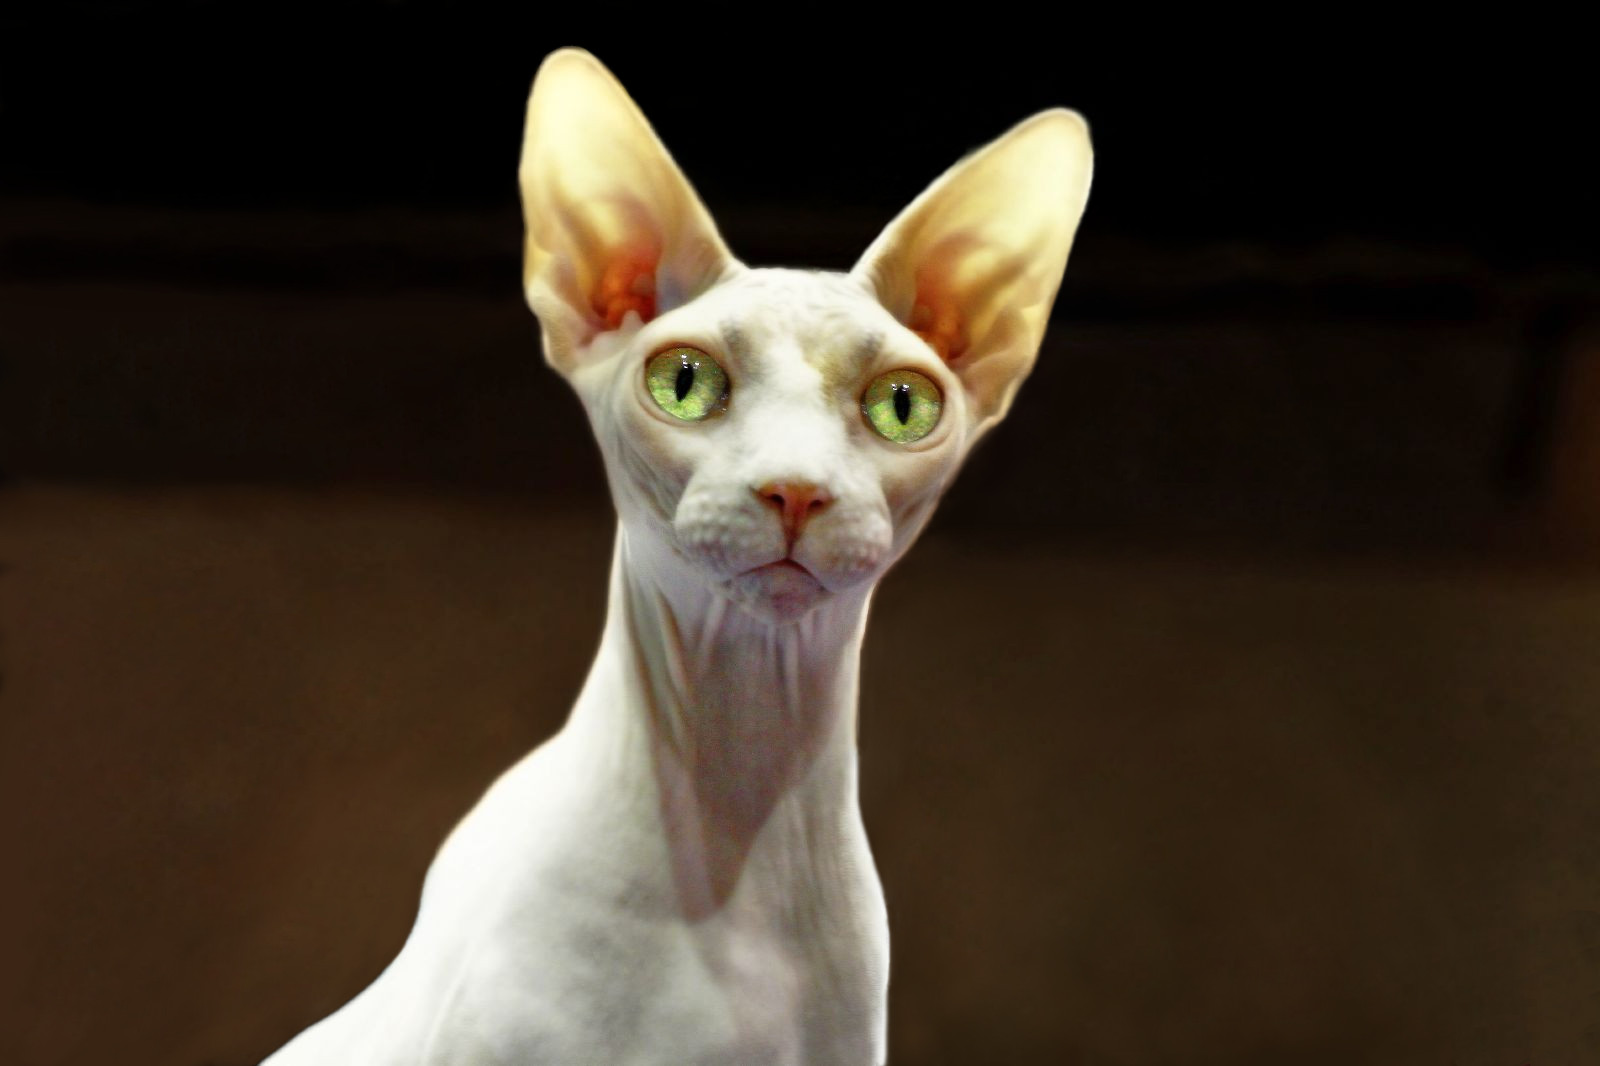
\includegraphics[width=0.7\textwidth]{images/cat.jpg}
	\caption{Eine Katze \cite{id}}
\end{figure}
ein text..

der ist gepastet. \cite{id}

\chapter{Hauptteil}

Nachstehend wird beschrieben, wie die Applikation entwickelt wurde.

\section{Softwaretechnologie}

Für die Entwicklung einer Applikation für den Web-Browser werden verschiedene Technologien benötigt, die jeweils für einen einzelnen Aspekt der Applikation verantwortlich sind.

\subsection{JavaScript}

JavaScript ist die Programmiersprache, die der Web-Browser unterstützt. Die Programmlogik wird in dieser Sprache geschrieben.

Viele Programmierer tendieren dazu, den JavaScript Code nach persönlicher Weise und auf nicht konsequente Weise zu formatieren, was die Lesbarkeit des Programmcodes, für den Autor als auch besonders für andere Betrachter, beeinträchtigt. Dies kann sich vor allem in umfangreichen Projekten, wo mehrere hundert Zeilen Code vorhanden sind, markant auf die Übersichtlichkeit auswirken. Da Open-Source von mehr und mehr praktiziert wird, gewinnen Syntaxkonventionen an Bedeutung. "`Das Anwenden der [Syntax-] Konvention bedeutet, die Syntaxkonventionen der Community und den Belang der Lesbarkeit des Programmcodes über die persönliche Programmierweise zu stellen"' \cite{feross}. Für bessere Programmqualität und Lesbarkeit wird deshalb in dieser Arbeit der \textit{JavaScript Standard Style} gebraucht, eine verbreitete Syntaxkonvention.

Diese Software verwendet die Programmierbibliothek \textit{Data-Driven-Documents (D3)}. Sie wurde von Michael Bostock, Vadim Ogievetsky und Jeffrey Heer erstellt und dient zur Entwicklung von Visualisationen im Web. Sie erleichtert die Benutzung des Document Object Models (DOM), ermöglicht effizienteres Debugging und verbessert die Leistung (\textit{"`Performance"'}) der Applikation \cite{bostock}.

%TODO three.js

\subsection{Hypertext Markup Language (HTML), Document Object Model (DOM)}

Hypertext Markup Language (HTML) ist in der Entwicklung einer Web-Applikation für den Inhalt (Text, Links, Bilder, Buttons...) der Seite zuständig. Die Sprache beschreibt durch \textit{Elemente}, die einen Wert haben können, verschachtelt sein können und denen \textit{Attribute} zugewiesen werden können die darzustellenden Informationen. 

Das Document Object Model (DOM) ermöglicht die dynamische Manipulation dieser Elemente durch Schnittstellen in JavaScript-Programmen.

\subsection{Scalable Vector Graphics (SVG)}

Scalable Vector Graphics (SVG) ist ein Format für Vektorgrafiken. SVG-Bilder bestehen nicht wie andere Bildformate (JPG, PNG) aus Pixeln, sondern aus Elementen wie Kreisen, Ellipsen, Rechtecke, Linien. SVG-Grafiken können im Browser dargestellt werden und durch JavaScript ebenfalls dynamisch manipuliert werden.

\subsection{Cascading Style Sheets (CSS)}

Cascading Style Sheets (CSS) beschreiben die Darstellung der anzuzeigenden Elemente, die in HTML-Dokumenten oder SVG-Grafiken vorkommen. CSS-Attribute können in HTML- oder SVG-Elementen im Attribut "`class"' durch \textit{Klassen} zugewiesen werden oder direkt im Attribut "`style"' definiert werden.
\section{Verarbeitung der Daten}

Bevor das Diagramm im Browser dargestellt werden kann, müssen zuerst die Daten geladen und verarbeitet werden. Die Beispiele dieser Arbeit nutzen ausschliesslich Datensätze, die frei verfügbar sind \cite{worldbank}.  %hier näher erklären TODO
Die Diagramme in Abbildung \ref{fig:scatterplot} benutzen einen Datensatz der Weltbank, der den $CO_2$-Verbrauch von Afghanistan beinhaltet.

%TODO beschreiben wieso ich diesen teil so ausführlich beschreibe. weil die datenverarbeitung überraschend schwierig umzusetzen war.darum will ich zeigen wieso.

Beim Prozess zur Veranschaulichung von Daten wird die \textit{Visualisierungspipeline} durchlaufen \cite[Kapitel 2.1]{viz}. Diese Pipeline stellt drei wesentliche Schritte des Prozesses dar: Die Datenaufbereitung (\textit{Filtering}), die Erzeugung des Geometriemodells (\textit{Mapping}) und die Bildgenerierung (\textit{Rendering}).

\subsection{Rohdaten}

\subsubsection{Comma-separated values (CSV)}

Die Applikation verwendet als Datenformat \textit{Comma-separated values} (\textit{CSV}). Das CSV-Format wird verwendet, um Tabellendaten zwischen Programmen auszutauschen \cite{csv}. Tabellenzeilen werden in der CSV-Datei durch einen Umbruch dargestellt, Spaltenwerte durch Kommas. Optional steht in der ersten Zeile (Abbildung \ref{fig:csv} links, Zeile 1) der Datei die Beschriftung der Spalten.

In Abbildung \ref{fig:csv} wird die Funktion des CSV-Formats demonstriert.

\begin{figure}[!htbp]
	\centering
	\begin{minipage}{0.5\textwidth}
		\centering
		\begin{minted}[linenos]{text}
Date,Value
2010-12-31,4220.717
2009-12-31,4352.729
2008-12-31,5555.505
2007-12-31,5067.794
		\end{minted}
	\end{minipage}\hfill
	\begin{minipage}{0.5\textwidth}
		\centering
		\begin{tabular}{ | l | l |}
			\hline
			\textbf{Date} & \textbf{Value} \\ \hline
			2010-21-31 & 4220.717 \\ \hline
			2009-21-31 & 4352.729 \\ \hline
			2008-21-31 & 5555.505 \\ \hline
			2007-21-31 & 5067.794 \\ \hline
		\end{tabular}
	\end{minipage}
	\caption[Demonstration des CSV-Formats]{Demonstration des CSV-Formats. Links: Die CSV-Datei in Rohtext. Rechts: Darstellung der Informationen der CSV-Datei in einer Tabelle.}
	\label{fig:csv}
\end{figure}

Man verwendet das CSV-Format oft, weil es sehr einfach aufgebaut ist. Das Lesen von solchen Tabellenformaten ist ohne grossen Aufwand in Programmen umsetzbar. 

Zudem beschränkt sich das CSV-Format nur auf die Vermittlung der Daten und beinhaltet keine Informationen zur Darstellung der Tabelle. Excel-Dateien (XLS/XLSX) hingegen speichern auch Daten zur Formatierung, auch Zeilengrösse, Textgrösse, Textformat und viele mehr. Für die Zwecke dieser Applikation sind diese Informationen irrelevant.
 
 
Wenn die Applikation die CSV-Datei laden und verarbeiten will, dann braucht sie zunächst zusätzliche Informationen zu der Datei: Die \textit{URL}, ein Zeichenstring, der eine über das Internet zugängliche Ressource repräsentiert \cite{url}.

Die Applikation lädt die Datei durch eine \textit{Ajax}-Anfrage (\textit{Asynchronous JavaScript and XML}) herunter, bevor sie sie weiter verarbeitet.

\subsection{Filtering}

Das Filtering ist der Prozess, der Rohdaten in aufbereitete Daten umwandelt. Die Aufgaben des Filtering sind zum Beispiel die Vervollständigung, Reduzierung oder Korrektur der Daten, sodass sie in den folgenden Schritten der Visualisierungspipeline verwendet werden können \cite[Kapitel 2.1]{viz}.

\subsubsection{Konvertierung in JavaScript-Objekte}

Als erster Schritt wird in der Applikation die CSV-Datei in \textit{JavaScript-Objekte} umgewandelt. Das Laden und \textit{Parsing} der Datei von CSV zu Objekten ist von D3 implementiert.

JavaScript-Objekte werden im \textit{JavaScript Object Notation}-Format (\textit{JSON}) dargestellt.

Im Abbildung \ref{fig:csv-json} ist der Prozess der Umwandlung ersichtlich: Es wird ein \textit{Array} von allen Zeilen in der Tabelle (ausgenommen der ersten Zeile, wo die Spalten beschriftet werden) erstellt. Jede Zeile wird als Objekt mit den dazugehörigen Spalten dargestellt.

\begin{figure}[!htbp]
	\centering
	\begin{minipage}{0.35\textwidth}
		\centering
		\begin{minted}[linenos]{text}
Date,Value
2010-12-31,4220.717
2009-12-31,4352.729
2008-12-31,5555.505
2007-12-31,5067.794
		\end{minted}
	\end{minipage}\hfill
	\begin{minipage}{0.55\textwidth}
		\centering

		\begin{minted}[linenos]{json}
[
  {
    "Date": "2010-12-31",
    "Value": "4220.717"
  },
  {
    "Date": "2009-12-31",
    "Value": "4352.729"
  },
  {
    "Date": "2008-12-31",
    "Value": "5555.505"
  },
  {
    "Date": "2007-12-31",
    "Value": "5067.794"
  }
]
		\end{minted}
	\end{minipage}
	\caption[CSV und JSON]{Konvertierung von CSV zu JavaScript Objekten. Links: CSV. Rechts: JSON.}
	\label{fig:csv-json}
\end{figure}

\subsubsection{Formatierung}

Die Applikation benötigt nun Anweisungen, um den Datensatz (im JSON-Format) zu formatieren, damit er im Diagramm verwendet werden kann. Der Prozess muss folgende Aufgaben erledigen (diese Strategie wurde selber entwickelt):

\begin{itemize}
	\item (Zeichenstring-) Elemente gegebenfalls in JavaScript-Objekte umwandeln
	\item Falls mehrere Datensätze vorhanden sind, diese \textit{mergen}, also in einen einzigen Array zusammenfassen
	\item Den gesamten gemergten Datensatz nach der unabhängigen Variable aufsteigend sortieren
\end{itemize}

\textbf{Umwandlung zu JavaScript-Objekten.} Das CSV-Format unterscheidet nicht zwischen Datentypen. Alle Werte in CSV-Dateien sind Zeichenstrings.

Im Beispiel in der Abbildung \ref{fig:csv-json} rechts, Zeile 3, wird für das erste Objekt im Array das Attribut mit dem Namen "`Date"' definiert. Der Datentyp ist hier ein Zeichenstring; damit ist eine Umwandlung in das JavaScript Date-Objekt, das ein Datum darstellt, sinnvoll: Das JavaScript Date-Objekt beherrscht viele Funktionen, wie zum Beispiel die Ausgabe der Anzahl Millisekunden, die seit dem 1. Januar 1970 vergangen sind. Dies ist beim Vergleichen von verschiedenen Date-Objekten nützlich. Das Date-Objekt ist zum Beispiel auch fähig, das Datum in einem Format auszugeben, das den lokalen Gegebenheiten entspricht: 28.10.2015 (Schweiz), 10/28/2015 (USA).

Zahlen, wie in Abbildung \ref{fig:csv-json} rechts, Zeile 4, im Attribut mit dem Namen "`Value"' definiert, werden zunächst von JavaScript als Zeichenstring behandelt. Diese Strings müssen in Zahlen-Objekte umgewandelt werden, denn nur mit Zahlen-Objekten können Rechenoperationen durchgeführt werden.

\textbf{Merging von Datensätzen.} Oft werden mehrere Datensätze in der Applikation geladen. Ein Beispiel ist der $CO_2$-Verbrauch von Ländern: Für jedes Land wird eine separate CSV-Datei geladen und in einen JavaScript-Array umgewandelt.

Es wurde entschieden, alle geladenen Datensätze (Arrays) in ein Datensatz (Array) zusammenzufassen (\textit{merge}), weil die Umsetzung aus Sicht der Programmierlogik einfacher ist. 

Da Spalten von verschiedenen Datensätzen meist mit gleichem Namen beschriftet sind, könnte man nach dem Merge die Spalten nicht unterscheiden (Abbildung \ref{fig:merge} oben). Darum wird die Beschriftung aller Spalten der abhängigen Variablen durch eine eindeutige Identifikation ersetzt (Abbildung \ref{fig:merge} unten). Die eindeutige Identifikation wird durch den Spaltennamen und die URL des Datensatzes generiert: Dem Spaltennamen wird ein Rautenzeichen und die URL angehängt. Dies ermöglicht, dass man trotz Merge die Objekte dem ursprünglichen Datensatz zuordnen kann.

In der Abbildung \ref{fig:merge} wurden zwei Datensätze mit den Dateinamen ch-co2.csv und af-co2.csv gemergt. Im unteren Beispiel wurden die Spaltennamen der abhängigen Variablen durch die eindeutige Identifikation ersetzt.

\begin{figure}[!htbp]
	\centering
	\begin{minipage}{0.40\textwidth}
		\centering
		\begin{minted}[linenos]{json}
[
  {
    "Date": "2010-12-31",
    "Value": "4220.717"
  },
  {
    "Date": "2009-12-31",
    "Value": "4352.729"
  },
  {
    "Date": "2010-12-31",
    "Value": "1320.717"
  },
  {
    "Date": "2009-12-31",
    "Value": "7353.129"
  }
]
		\end{minted}
	\end{minipage}\hfill
	\begin{minipage}{0.5\textwidth}
		\centering
		\begin{minted}[linenos]{json}
[
  {
    "Date": "2010-12-31",
    "Value#ch-co2.csv": "4220.717"
  },
  {
    "Date": "2009-12-31",
    "Value#ch-co2.csv": "4352.729"
  },
  {
    "Date": "2010-12-31",
    "Value#af-co2.csv": "1320.717"
  },
  {
    "Date": "2009-12-31",
    "Value#af-co2.csv": "7353.129"
  }
]
		\end{minted}
	\end{minipage}
	\caption[Merge-Strategie]{Demonstration der Merge-Strategie und Anwendung der ID-Generierung. Oben: Gemergter Datensatz, ohne eindeutige IDs. Unten: Gemergter Datensatz, mit eindeutigen IDs.}
	\label{fig:merge}
\end{figure}

\textbf{Sortieren des gemergten Datensatzes.} Der Datensatz wird nach der unabhängigen Variable ansteigend sortiert, damit die Berechnung von Interpolationen ermöglicht wird.

\subsubsection{Datensatzspezifische Filteringkonfiguration und Hard Coding}

Die Applikation soll fähig sein, mehrere Formate von CSV-Datensätzen verarbeiten zu können. Der Benutzer sollte die Anweisungen zum Filtering anpassen können.

Die Implementation dieser Anweisungen zum Filtering (Spezifikation der URLs, abhängige und unabhängige Variablen, Datentypen der Spalten des Datensatzes) kann auf zwei Arten durchgeführt werden:

\begin{itemize}
	\item Die Anweisungen zum Filtering sind im Sinne des \textit{Hard Coding} implementiert
	\item Die Anweisungen zum Filtering sind in einer \textit{Konfiguration} abgelegt (\textit{Soft Coding})
\end{itemize}

\textbf{Hard Coding.} Die Anweisungen (Konfiguration) zum Filtering sind direkt im Programmcode abgelegt. Falls Datensätze mit anderen URLs, Spaltennamen oder Datentypen in der Applikation verwendet werden sollen, so müssen die Anweisungen direkt im Programmcode entsprechend angepasst werden.

\textbf{Soft Coding.} Beim Soft Coding sind die Anweisungen (Konfiguration) für das Filtering in einer externen Ressource abgelegt, zum Beispiel in einer Datei oder Datenbank. Die Applikation liest die Konfiguration und führt das Filtering dementsprechend aus. Dem Benutzer ist es so möglich, die Funktionsweise der Applikation anzupassen. Soft Coding wird in dieser Applikation verwendet.

\subsubsection{meta.json}

Die Applikation verwendet als Konfiguration eine Datei im JSON-Format, die vor dem Filtering in ein JavaScript-Objekt umgewandelt werden kann. In Abbildung \ref{fig:meta} ist ein Beispiel der Konfigurationsdatei meta.json aufgelistet:

\begin{itemize}
	\item \texttt{dataset} (Zeile 3-22) beschreibt ein Datensatz
	\item \texttt{url} (Zeile 4) gibt die URL des Datensatzes an
	\item \texttt{config} (Zeile 5-21) ist ein Array, in dem die Spalten des Datensatzes konfiguriert werden
	\item \texttt{row} (Zeile 7, 14) gibt die zu konfigurierende Spalte an
	\item \texttt{type} (Zeile 8, 15) hat entweder den Wert \texttt{index} oder \texttt{value}. \texttt{index} bedeutet, dass die Spalte eine unabhängige, \texttt{value} bedeutet, dass die Spalte eine abhängige Variable ist
	\item \texttt{data\_type} (Zeile 9, 16) gibt den Datentyp der Spalte an, damit sie in das entsprechende JavaScript-Objekt umgewandelt werden kann. Er kann den Wert \texttt{Date} oder \texttt{Number} haben
	\item \texttt{date\_format} (Zeile 10) gibt bei Spalten mit Datentyp \texttt{Date} das Format des Datums an, damit es geparst werden kann
	\item \texttt{name} (Zeile 11, 17) setzt einen Namen für den Datensatz, der im Diagramm angezeigt werden soll
	\item \texttt{activated} (Zeile 18) gibt an, ob der Datensatz standardmässig im Diagramm angezeigt werden soll. Dieses Attribut spielt besonders eine Rolle bei Diagrammen, die mehrere Datensätze darstellen
	\item \texttt{unit} (Zeile 19) stellt die Einheit einer abhängigen Variablen dar. Sie wird als Information im Diagramm angezeigt
\end{itemize}

\begin{figure}[!htbp]
	\centering
	\begin{minted}[linenos]{json}
{
  "datasets": [
    {
      "url":"data/WWDI-AFG_EN_ATM_CO2E_KT.csv",
      "config": [
        {
          "row": "Date",
          "type": "index",
          "data_type": "Date",
          "date_format": "%Y-%m-%d",
          "name": "Datum"
        },
        {
          "row": "Value",
          "type": "value",
          "data_type": "Number",
          "name": "Afghanistan",
          "activated": true,
          "unit": "kt"
        }
      ]
    }
  ]	
}
	\end{minted}
	
	
	\caption[Beispiel der Konfigurationsdatei: meta.json]{\textbf{meta.json}: Beispiel der Konfigurationsdatei, die die Applikation verwendet.}
	\label{fig:meta}
\end{figure}

\subsection{Mapping}

Das Mapping ist der Prozess der Umwandlung von aufbereiteten Daten zu Geometriedaten, es ist das Kernstück der Diagrammerstellung. Es wird eine \textit{Daten-zu-Geometrie-Abbildung} realisiert \cite[Kapitel 2.1]{viz}.

In der Applikation, die in dieser Arbeit entwickelt wird, stellen die Geometriedaten die SVG-Elemente wie zum Beispiel Rechtecke, Kreise, Linien, Text dar.

Die Programmlogik des Mappings unterscheidet sich grundlegend bei jedem Diagrammtyp. In dieser Arbeit werden mehrere Typen von Diagrammen entwickelt, der Prozess des Mappings wird daher für jeden Typ separat behandelt.

\subsection{Rendering}

% geometriedaten -> bilddaten

Das Rendering ist der letzte Schritt der Diagrammerstellung, bei dem die Abbildung der Geometriedaten in Bilddaten erfolgt \cite[Kapitel 2.1]{viz}.

In unserem Falle sind Bilddaten das Diagramm, das im Browser angezeigt wird. Es ist die Aufgabe des Browsers, die Geometriedaten (SVG-Elemente) mit Darstellungsanweisungen (CSS) in Bilddaten (Pixel, angezeigte Grafik) zu rendern.

\section{Information-Seeking Mantra}

Als Startreferenz für die Entwicklung des interaktiven Diagrammes bieten sich die von Ben Shneiderman begründeten Prinzipien für das Design graphischer Benutzeroberflächen an, das "`\textit{Information-Seeking Mantra}"'. Die Weise, wie der Benutzer mit der Oberfläche interagiert, hat Shneiderman \cite{shneiderman} festgelegt:

\begin{itemize}
	\item Überblick ("`\textit{Overview first}"')
	\item Zoomen und Filtern ("`\textit{zoom and filter}"')
	\item Details auf Abruf ("`\textit{then details-on-demand}"')
\end{itemize}

\textbf{Überblick.} Der Benutzer verschafft sich einen Überblick über die gesamte Oberfläche des Programms.

\textbf{Zoom.} Zur besseren Betrachtung vergrössert der Benutzer die Ansicht, sodass die betreffenden Elemente grösser angezeigt werden.

\textbf{Filter.} Die Filter-Funktion ermöglicht dem Benutzer, gewisse Elemente oder Elementgruppen je nach Interesse ein- oder auszublenden.

\textbf{Details auf Abruf.} Falls ein Element den Nutzer besonders interessiert, besteht die Möglichkeit, dass zusätzliche relevante Informationen zum Element angezeigt werden können.

Zusätzlich formulierte Shneiderman drei weitere Schritte:

\textbf{Zusammenhänge betrachten.} Die Zusammenhänge zwischen den verschiedenen Elementen können im Programm betrachtet werden. Diesen Schritt umzusetzen ist nur bei wenigen Benutzeroberflächen sinnvoll, zum Beispiel bei der Darstellung von Baumdiagrammen oder anderen Diagramme mit hierarchischen Daten.

\textbf{Verlauf.} Die Interaktionen des Benutzers mit der Programmoberfläche werden aufgezeichnet. Dadurch können Interaktionen rückgängig gemacht werden.

\textbf{Extraktion.} Damit wird die Extraktion erlaubt der \textit{Query-Parameter} (wie angewandte Filter, Verlauf, Zoomstufe) und der durch die Interaktion bereits definierten Elementgruppen ("`\textit{subcollections}"').

Im Diagramm werden nur die Methoden \textit{Überblick}, \textit{Zoom}, \textit{Filter} und \textit{Details auf Abruf} umgesetzt. Das Mantra wurde allgemein für Benutzeroberflächen von Programmen beschrieben, in unserer Applikation, einem interaktiven Diagramm, macht aber die Umsetzung der Schritte \textit{Zusammenhänge betrachten}, \textit{Verlauf}, \textit{Extraktion} in Bezug auf die Funktion des Diagramms keinen Sinn:

\begin{itemize}
	\item Punktediagramme oder Liniendiagramme werden nicht dazu verwendet, Daten in Hierarchieform darzustellen.
	\item Die Interaktionen im Diagramm sind zu banal, als dass eine Rückgängig-Funktion von Nutzen wäre.
	\item Die Extraktion und der Export von Query-Parametern des Diagramms ist zwar theoretisch umzusetzen, ist jedoch von minimaler praktischer Bedeutung.
	\item Zur Extraktion von "`\textit{subcollections}"' aus einem Datensatz sollte kein interaktives Diagramm verwendet werden. Eine Datenverarbeitungsapplikation ist für diese Aufgabe angemessener, da exakte Parameter zur Extraktion bestimmt werden können.
\end{itemize}
\section{Zweidimensionales Punktdiagramm}

Da das zweidimensionale Punktdiagramm weit verbreitet ist, sind sich Betrachter an diese Darstellung gewöhnt. Oft werden die Punkte in Diagramm durch eine Linie verbunden, was den Verlauf der abgebildeten Datenwerte verdeutlicht, besonders in Medien, zum Beispiel für die Darstellung von Börsenkursen. 

Aus diesem Grund wurde als erstes Beispiel das zweidimensionale Punktdiagramm (beziehungsweise das Liniendiagramm, falls Linien hinzugefügt werden) ausgewählt.


\subsection{Applikation}

\begin{figure}[!htbp]
	\centering
	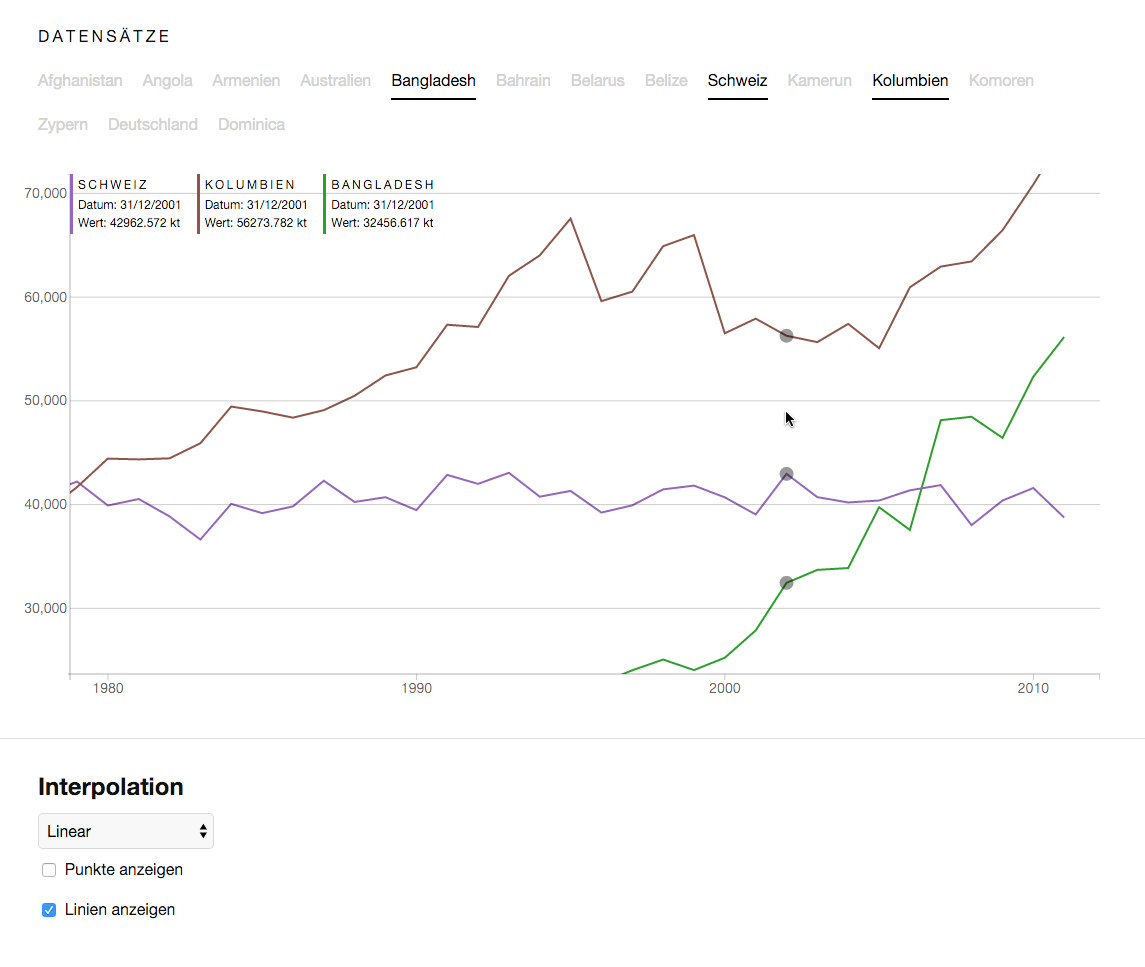
\includegraphics[width=\linewidth]{images/2dline}
	\caption{Screenshot der Oberfläche der Applikation (zweidimensionales Liniendiagramm/Punktdiagramm)}
	\label{fig:screenshot}
\end{figure}

Der Screenshot in Abbildung \ref{fig:screenshot} zeigt die entwickelte Applikation. Es sind Datensätze \cite{worldbank} zum $CO_2$-Verbrauch von 15 Ländern vorhanden, drei davon sind im Diagramm eingeblendet. Der Name des Tests in der Applikation lautet \texttt{layout}.

\textbf{Achsen.} Es wurden Achsen mit linearer Skala für die Applikation gewählt. Beschriftungen und Markierungen, sogenannte \textit{Ticks}, sind vorhanden. Die Ticks auf der Ordinatenachse (y-Achse) wurden in Richtung der Innenseite des Diagramms verlängert, so dass ein Gitter entsteht.

Falls in einem Diagramm mehrere Datensätze gleichzeitig dargestellt werden sollen, wie es der Fall in Abbildung \ref{fig:screenshot} ist, so müssen die abgebildeten Werte die gleiche Einheit (zum Beispiel Meter, Kilogramm, Franken) besitzen. Bei der gleichzeitigen Darstellung von mehreren Datensätzen mit verschiedenen Einheiten in einem Diagramm muss für jede vorhandene Einheit eine eigene Achse und Skala gezeichnet werden.

\textbf{Datenpunkte.} Die Applikation bietet an, die Daten als Punkte und bzw. oder verbunden durch eine Linie anzuzeigen. In Abbildung \ref{fig:screenshot} unten wird durch Kontrollkästchen ermöglicht, die Anzeige zu verändern.

\textbf{Layout und Textformatierung.} Für den Schritt \textit{Übersicht} ist das Layout und auch die Formatierung des Textes von Bedeutung. Eine klare Oberflächenstruktur nach modernen Minimalismus (nach Designtrends wie \textit{Flat Design} oder \textit{Material Design}) wurde geschaffen, bei denen der Inhalt im Vordergrund steht. "`Benutzer betrachten keine Details, sie benutzen Details."' \cite{minimalism}.

Zur besseren Orientierung des Benutzers wird hier das Prinzip von "`\textit{pop}"' und "`\textit{unpop}"' von Text, das von Erik Kennedy \cite{pop} beschrieben wurde, berücksichtigt: Durch die Anpassung der Typographie kann ein Text hervorgehoben beziehungsweise in den Hintergrund gestellt werden. Folgende Eigenschaften von Texten im Diagramm werden in der Applikation entsprechend der Wichtigkeit angepasst:

\begin{itemize}
	\item Grösse (grösser bzw. kleiner)
	\item Farbe (grösserer bzw. kleinerer Kontrast)
	\item Schriftstärke (fetter bzw. leichter)
	\item Schriftart (Grossschreibung bzw. Kleinschreibung)
	\item Laufweite (kleiner bzw. grösser)
	\item Unterstreichung (unterstrichen bzw. nicht unterstrichen)
\end{itemize}

\textbf{Linien.} Der Verlauf der abgebildeten Datenwerte wird verdeutlicht, indem die Punkte im Diagramm durch eine Linie verbunden werden. Die lineare Interpolation wurde durch ein selbstgeschriebenes Modul implementiert. Weitere Interpolationen, wie der \textit{Kubisch Hermitescher Spline} oder \textit{Basis-Spline}, wurden mit D3 implementiert und können auf das Diagramm angewendet werden.

\begin{figure}[!htbp]
	\begin{minipage}{\textwidth}
		\centering
		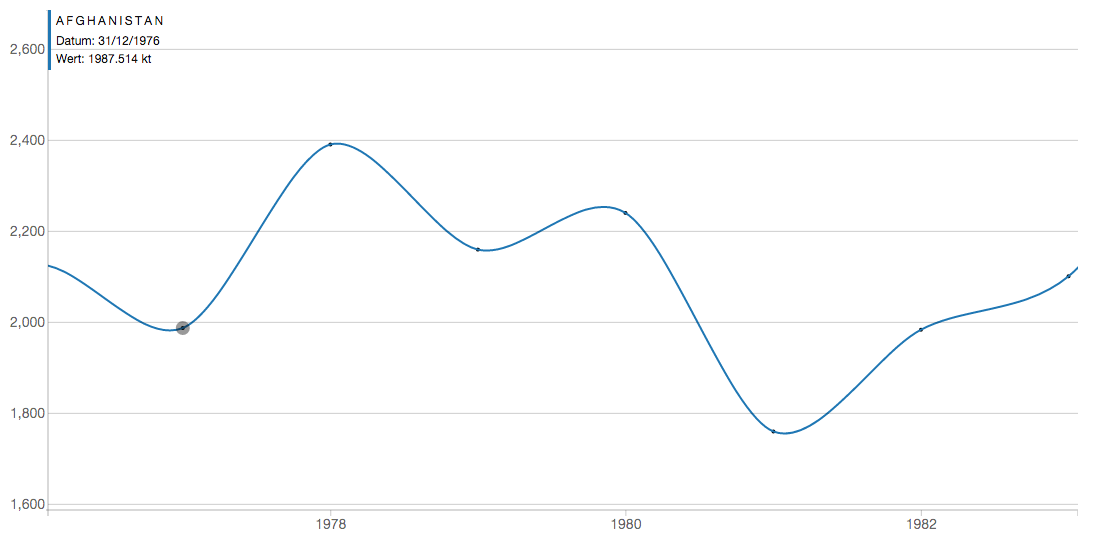
\includegraphics[width=\linewidth]{images/cardinal}
	\end{minipage}
	\begin{minipage}{\textwidth}
		\centering
		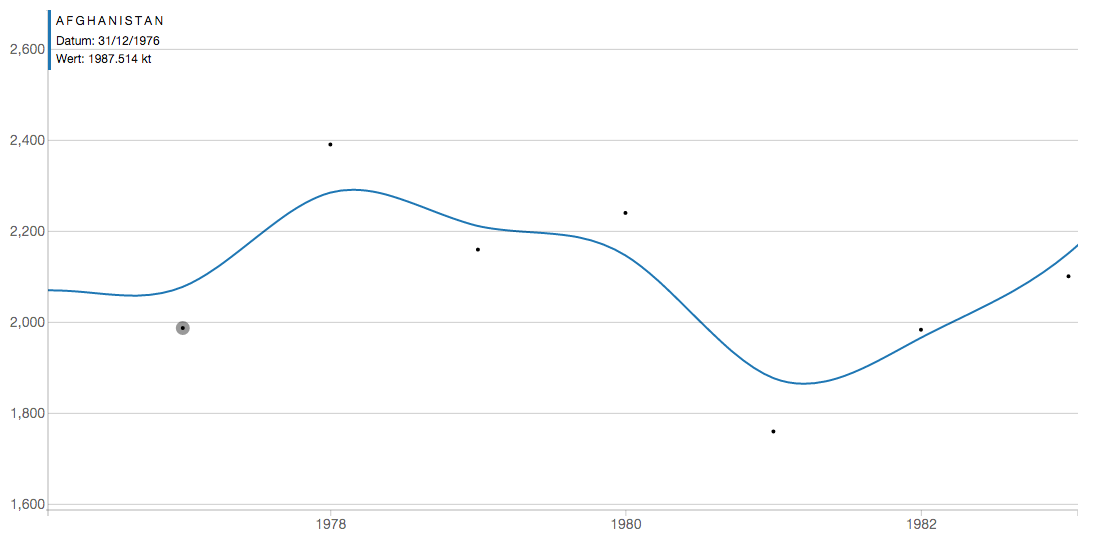
\includegraphics[width=\linewidth]{images/basis}
	\end{minipage}
	\caption[Beispiele von Interpolationen und Zoom]{1. Beispiele von Interpolationen im Diagramm. V.o.n.u: Kubisch Hermitescher Spline, Basis-Spline. 2. Gezoomte Ansicht}
	\label{fig:vergleich}
\end{figure}

Verschiedene Farben von Linien ermöglichen die Zuordnung von Datensätzen. Die den Datensätzen zugewiesenen Farben werden in der Detailanzeige dargestellt.

\textbf{Zoom.} Der Schritt \textit{Zoomen} wurde im Diagramm umgesetzt. Es kann durch Scrollen gezoomt werden, indem die Skalierungen der Achsen verändert werden. Die Programmlogik wurde mittels D3 implementiert. 

Es gibt zahlreiche interaktive Diagramme, in denen nur der Zoom durch Veränderung der Skalierung der Abszisse möglich ist. Dabei wird nach jedem Zoom-Vorgang die Skalierung der Ordinate and die Daten neu angepasst oder überhaupt nicht verändert.

Diese Zoom-Strategie verwirrt den Benutzer, weil sich die Skalierungen der Achsen nicht gleichmässig beim Zoom verändern: Er nimmt ein Dehnen bzw. Zusammendrücken des Diagramms wahr. Der Benutzer ist es sich gewöhnt, dass die beiden Skalierungen stets im gleichen Verhältnis stehen; dies ist auch beim Zoom bei Smartphones üblicherweise der Fall. Deshalb wurde diese Zoomstrategie bevorzugt und umgesetzt.

\textbf{Datensatzauswahl.} In diesem Beispiel (Abbildung \ref{fig:screenshot}) können Linien ein- und ausgeblendet werden, die Datensätzen für 15 Länder entsprechen. Dieser Vorgang gehört zum Schritt \textit{Filtern}. Aktivierte, angezeigte Datensätze werden nach den Prinzipien von Kennedy hervorgehoben, nicht aktivierte, versteckte Datensätze sind in den Hintergrund gestellt.

\textbf{Tooltip und Detailanzeige.} Beim Tooltip wird der der Maus am nächsten liegende Datenpunkt jedes Datensatzes markiert und erscheint in der Detailanzeige. In der Detailanzeige werden, falls im Datensatz vorhanden, weitere Informationen (Datenspalten) und genaue x- und y-Werte mit Einheit angezeigt. Dieser Vorgang entspricht dem Schritt \textit{Details auf Abruf}.

\textbf{Dynamik der Applikation.} Der Screenshot dieses Beispiels (Abbildung \ref{fig:screenshot}) ist das Resultat der Anzeige der Applikation, die für einen bestimmten Datensatz konfiguriert ist. Elemente des Diagramms, wie der Wertebereich der Achsen, die Datensatzauswahl, Tooltip und Detailanzeige, werden dynamisch generiert, so dass diese Module ohne weitere Einstellung auch für andere Datensätze funktionieren.


\section{Dreidimensionales Punktediagramm}

Falls Datensätze mit einer unabhängigen und zwei abhängigen Variablen dargestellt werden sollen, kann ein dreidimensionales Punktediagramm verwendet werden.
\section{N-dimensionales Punktdiagramm}

Falls man einen Datensatz darstellen will, der mehr als zwei unabhängige Variablen enthält, so kann die Darstellung in einem n-dimensionalen Punktdiagramm umgesetzt werden.

Datensätze in einem n-dimensionalen Merkmalsraum können in 2-dimensionalen Merkmalsräumen veranschaulicht werden und so gruppiert werden, dass eine Gesamtansicht auf die Daten möglich sind: In einer Scatterplot-Matrix \cite{viz}.

Als Versuchsdaten wurden Datensätze der World Bank \cite{worldbank} zur Bevölkerung, Arbeitsplätze und GDP der Schweiz im Verlauf der Zeit verwendet.

Ein n-dimensionales Punktdiagramm wurde im Test \texttt{dimensions} umgesetzt, sodass Datensätze mit der entsprechenden Konfigurationsdatei \texttt{meta.json} dargestellt werden können (Abbildung \ref{fig:nd}). Es wurde jedoch schnell erkannt, dass sich diese Art von Punktdiagramm nicht als interaktives Diagramm eignet:

\begin{itemize}
	\item Die Elemente der Scatterplot-Matrix hängen nicht zusammen. Die Achsen jedes Elements haben eine eigene Skalierung, darum ist die Umsetzung von Zoom, Tooltip, Detailanzeige so unmöglich.
	\item Ein weiterer Nachteil, der allerdings nicht mit der Interaktion zusammenhängt: Das Zustandekommen der einzelnen Scatterplots ist für den Benutzer nicht offensichtlich.
\end{itemize}

\begin{figure}[!htbp]
	\centering
	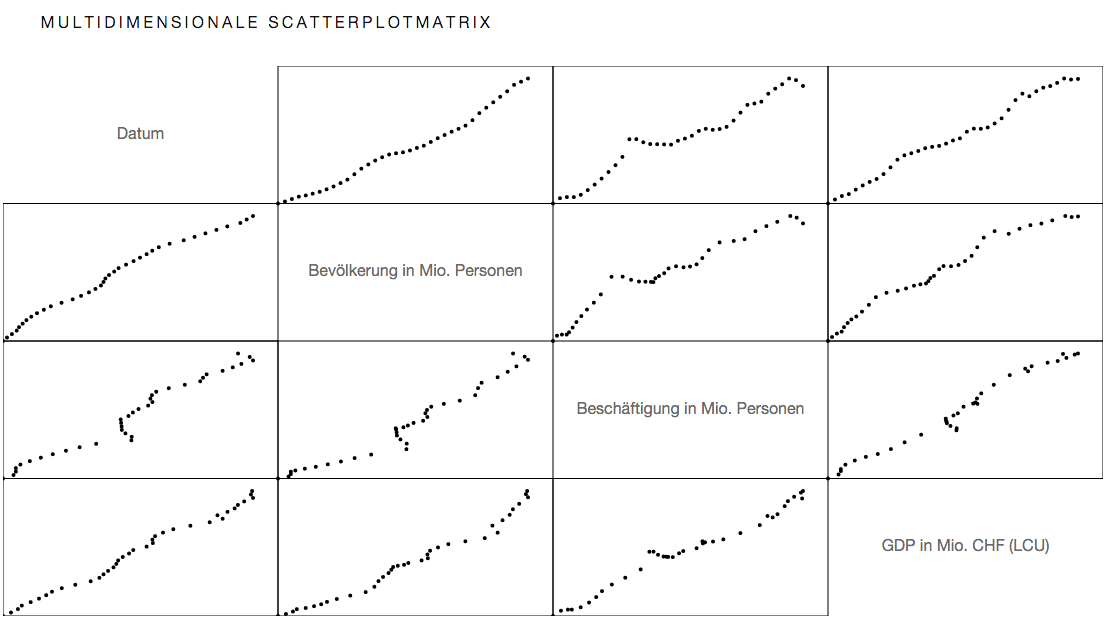
\includegraphics[width=\linewidth]{images/nd}
	\caption{Screenshot der Oberfläche der Applikation (n-dimensionales Punktdiagramm)}
	\label{fig:nd}
\end{figure}

\chapter{Schlusswort}

Durch Umsetzung von verschiedenen Interaktionsmethoden an selbstentwickelten Diagrammen konnte die Analyse und das Verständnis gegenüber der statischen Version verbessert werden.

Neben der Dokumentation des Entwicklungsprozesses und der verwendeten Technologien wurde für die interaktiven Diagramme eine optimale Datenverarbeitungsstrategie entwickelt (siehe "`Merge"' und "`meta.json"'). Dabei wurde auch viel Wissen über JavaScript im Allgemeinen, JavaScript Buildsysteme (NPM, Gulp.js, Browserify), Open Source, Web Design (CSS, Minimalismus, Pop/Unpop) und über den Umgang mit Programmbibliotheken (D3, three.js, tween.js) erarbeitet.

Was den Entwicklungprozess der Applikation und das Verfassen des Codes betrifft, wurden folgende Erkenntnisse gewonnen: Bei Projekten mit einer solchen grossen Menge Code ist es sehr wichtig, Teile zu abstrahieren. Diese Abstraktion konnte mittels \textit{Modulen} (Browserify) erzielt werden.

Beim zweidimensionalen Punkt-/Liniendiagramm wurden Möglichkeiten für die Interaktion mit Benutzeroberflächen entsprechend implementiert: Zoom, Tooltip, Detailanzeige und Datensatzauswahl. Es wurde so auch erreicht, dass Benutzer sich mit einer grossen Datenmenge effizienter auseinandersetzen können. 

Zudem wurden Diagrammtechniken implementiert wie Achsen, Skalierungen und Interpolationen. Die Theorie hinter diesen Möglichkeiten und Techniken sind ebenfalls in der Arbeit dokumentiert worden.
\newpage
Eine unkonventionelle Weise der Darstellung eines Datensatzes mit zwei abhängigen Variablen, das dreidimensionale Diagramm, wurde erläutert und als Applikation umgesetzt. Eine Methode wurde dazu entwickelt, welche die Benutzung des Diagramms produktiver machen sollte: Parallelprojektionen, die das dreidimensionale Punktdiagramm auf zweidimensionale Punktdiagramme reduzieren können.



\newpage
%now enable appendix numbering format and include any appendices
\appendix

%next line adds the Bibliography to the contents page
%\renewcommand{\bibname}{Literatur}
\chapter{Literatur}
\printbibliography[heading=none]     %use a bibtex bibliography file refs.bib

\newpage
\chapter{Abbildungsverzeichnis}
\makeatletter
\@starttoc{lof} % Print List of Figures
\makeatother

\newpage
\chapter{Bestätigung der Eigenständigkeit}
Der Unterzeichnete bestätigt mit Unterschrift, dass die Arbeit selbständig verfasst und in schriftliche Form gebracht worden ist, dass sich die Mitwirkung anderer Personen auf Beratung und Korrekturlesen beschränkt hat und dass alle verwendeten Unterlagen und Gewährspersonen aufgeführt sind.

\end{document}